% !TeX root = ../paper.tex
% !TeX encoding = UTF-8
% !TeX spellcheck = en_US

\section{Self-Healing}\label{sec:self-healing}
  Self-healing is an integral part of self-adaptive systems and the focus of this paper.
  It combines properties of
  (i) fault-tolerant systems, which handle transient failures and mask permanent ones to ensure system availability,
  (ii) self-stabilizing systems, which are non-fault masking and converge to the legal state in a finite amount of time, and 
  (iii) survivable systems, which maintain essential services and recover non-essential ones after intrusions have been dealt with~\cite{PsaierSurvey}.
  A widely-used definition for self-healing systems is from \citeauthor{Ghosh}~\cite{Ghosh}:

  \begin{quote}
    The key focus [...] is that a self-healing system should recover from the abnormal (or \enquote{unhealthy}) state and return to the normative (\enquote{healthy}) state, and function as it was prior to disruption.
  \end{quote}

  This definition is very broad, but one can argue that the key aspect of self-healing systems are recovery oriented functionalities that bring the system back to the healthy state, which neither sole fault-tolerant systems nor sole survivable systems encompass~\cite{PsaierSurvey}.

  Like in an autonomous system, the main component in a self-healing system is the self-healing manager.
  It runs a control loop with three stages that is a reduced version of the autonomic control loop, also referred to as MAPE-K loop~\cite{ibm_autonomic}.
  The self-healing loop consists of the following three main stages~\cite{PsaierSurvey}:

  \begin{description}
    \item[Detect] The self-healing manager filters the status information about the running system and reports suspicious events and detected degradations.
    \item[Diagnose] The diagnosis stage performs root cause analysis on the received reports from the previous stage and calculates a recovery strategy.
    \item[Recover] In the recovery phase the manager applies the strategies to the system while he avoids any unpredictable side effects.
  \end{description}

  \begin{figure}
    \centering
    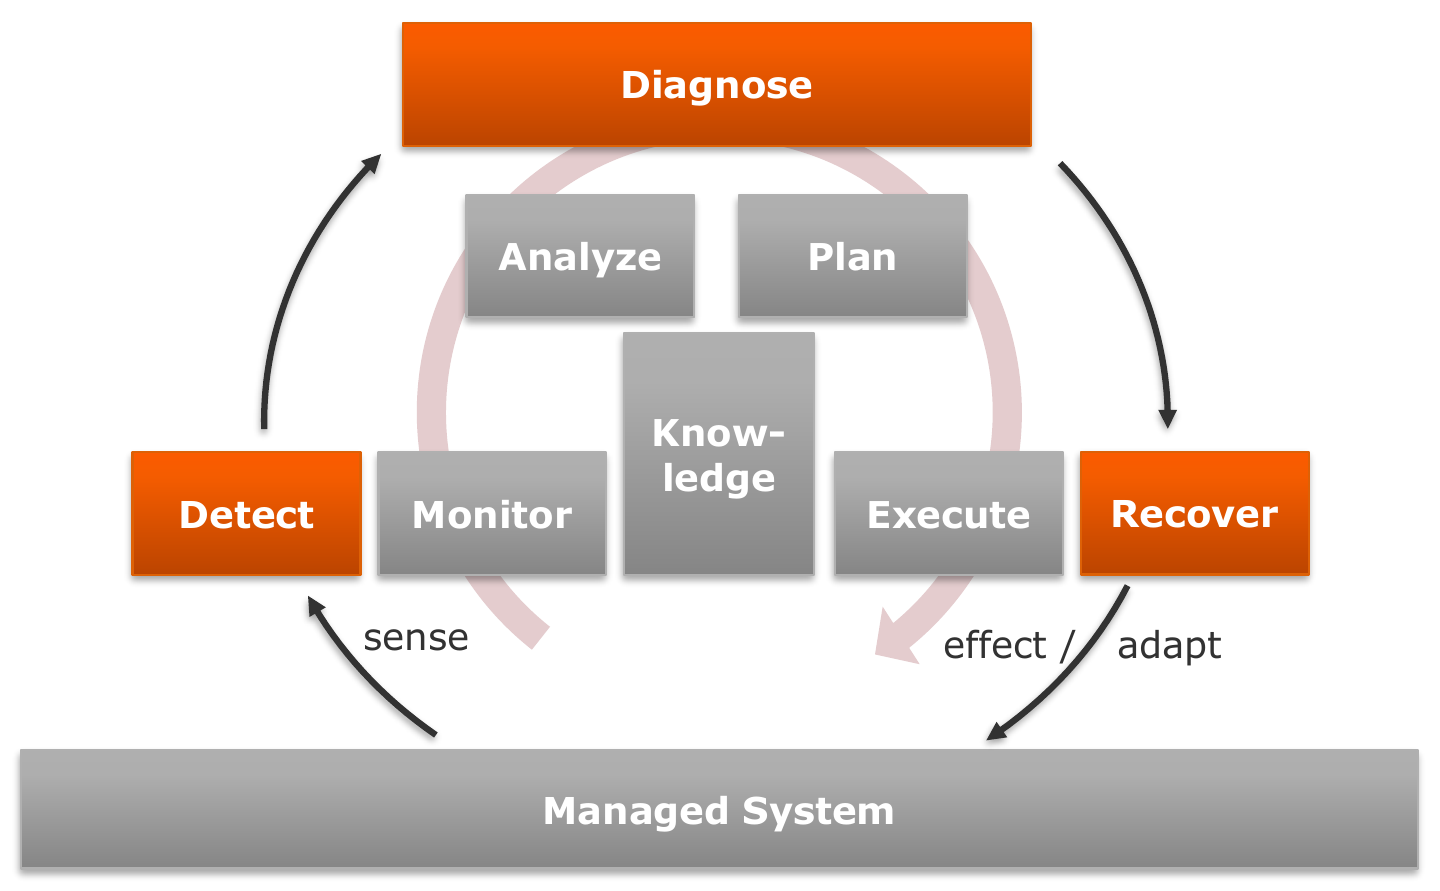
\includegraphics[width=\linewidth]{reduced-control-loop}
    \caption{Condensed autonomic control loop as the self-healing loop}
    \label{fig:self-healing-loop}
  \end{figure}

  These three stages reflect the definition of self-healing.
  There are different ways, how a software system can be equipped with the above mentioned self-healing capabilities.

  The first approach is a software application with built-in self-healing logic.
  This means that the self-healing manager is within the application code and is able to access internal state and mechanisms.
  This can be an advantage as the application is a white box and the self-healing logic can use detailed status information and even domain knowledge for detection, analysis and recovery.
  At the other hand, this also means that the healing logic is tied to the application increasing coupling and violating the separation of concerns principle.
  If the application starves the self-healing manager may starve as well.

  The second approach is an external self-healing manager provided as an infrastructural component or as third-party service.
  The self-healing logic runs in isolation from the application code and can therefore treat the application only as a black box and has to use external metrics to judge the application's health.
  It's the current state of the art for monitoring, health management and scaling logic~\cite{ToffettiMicroservices}.
  The external management logic has to be themselves resilient, fault-tolerant, and scalable for being able to heal the application.
  Using third party services or services provided by the infrastructure provider could lead to vendor lock-in.
  There are also open-source alternatives that can be used as middleware between cloud infrastructure and the application, such as \gls{kubernetes}.

  \subsection{Architecture-based self-healing}
  \begin{itemize}
    \item introduce related work: research approaches to self-healing:
    \item \cite{DashofyArchitecture}
    \begin{itemize}
      \item architecture-based approach
      \item $\rightarrow$ repairs are done on the level of software components or connectors
      \item external to application
      \item targets event-based software architectures
    \end{itemize}
    \item This approach
    \begin{itemize}
      \item microservice container orchestrator approach
      \item $\rightarrow$ repairs are done on container-level
      \item external to application (\gls{kubernetes})
      \item targets microservice architectures deployed in cloud environments using containers and \gls{kubernetes}
    \end{itemize}
  \end{itemize}

\subsection{Self-healing challenges in cloud environments}
  While systems and software components can fail in various ways and research has come up with general failure classifications and resolutions~\cite[Tab.~1]{PsaierSurvey}, failures in cloud environments can be reduced to one failure: a node or component is detected unreachable.
  Although an unreachable node can have different root causes on the infrastructure level, the impact on the system is the same and we have no control about the infrastructure in a cloud deployment.
  This means that we have to find other ways besides repairing the infrastructure to heal from those failures.
  Node failures can be detected via heartbeat messages or latency metrics and a common recovery strategy used is the restart of the software that was running on the node on another node.

  \begin{quote}
    In the pre-cloud days, this would have been pretty manual, some poor sap of an engineer would have to nurse a bare metal or VM back to health.
    Now, with cloud-based abstractions, individual compute units are much more expendable.
    We can just take them down and replace them with new ones.
  \end{quote}

  \begin{itemize}
    \item Reactive Manifesto~\cite{reactivemanifesto} asks for more resilient and responsive systems.
    The resilience is achieved by replication, containment, isolation, and delegation.
    Recovery should be handled by an external component.
    This could be a self-healing component.
    \item \cite{StackCloud}
      \begin{itemize}
        \item hierarchical approach
        \item layered master-slave architecture to provide flexibility and high availability
        \item targets decentralized cloud architectures
      \end{itemize}
    \item \cite{gru}
      \begin{itemize}
      \item similar to this approach, but they have developed their own container orchestration tool, called Gru, instead of using \gls{kubernetes}
      \item also targets microservice architectures deployed in containers
    \end{itemize}
  \end{itemize}

\subsection{Self-healing microservices}
  \citeauthor{ToffettiMicroservices} propose such (application with built-in self-healing logic) a system for a microservice architecture.
  They leverage standard methods from distributed systems (\ie consensus algorithms) to assign self-management (includes self-healing) functionality to some nodes of the distributed application.
  The selected nodes form a hierarchy and perform different parts of the self-management logic.
  This means that the self-management logic is distributed in the cluster to overcome the connectedness to the application code.

  \begin{itemize}
    \item \cite{ToffettiMicroservices}
    \item architecture-based approach
    \item self-managing microservice applications
    \item within application
    \item targets microservice applications
  \end{itemize}

\section[Kubernetes]{\gls{kubernetes}}\label{sec:kubernetes}
  % https://kubernetes.io/docs/concepts/overview/what-is-kubernetes/
  \Gls{kubernetes} is an open-source platform for automating and managing distributed software in the cloud.
  It heavily relies on container technology and supports the declarative configuration of the managed containers.
  \Gls{kubernetes} was developed by Google and is open-source software since 2014~\cite{kubernetes}.

  % https://kubernetes.io/docs/concepts/overview/components/
  \Gls{kubernetes} is build on top of existing \gls{paas} solutions and consists of a master-slave architecture forming a cluster.
  Slave nodes, \gls{kubernetes} calls them only nodes, are responsible for executing and maintaining the actual application via an underlying container runtime.
  Most of the time Docker~\cite{docker} is used.
  The nodes also run \gls{kubernetes} components that manage cluster networking (\texttt{kube-proxy}) and interact with the container runtime and the master to monitor and manage the pods of the local node (\texttt{kubelet}).
  % https://kubernetes.io/docs/concepts/workloads/pods/pod-overview/
  Pods are the smallest deployment unit in \gls{kubernetes} and consist of the application container (or multiple), connected resources, such as storages or network addresses, and the configuration options.
  The container runtime, \texttt{kube-proxy} and \texttt{kubelet} form the \gls{kubernetes} runtime environment~\cite{kubernetes}.

  \begin{figure}
    \centering
    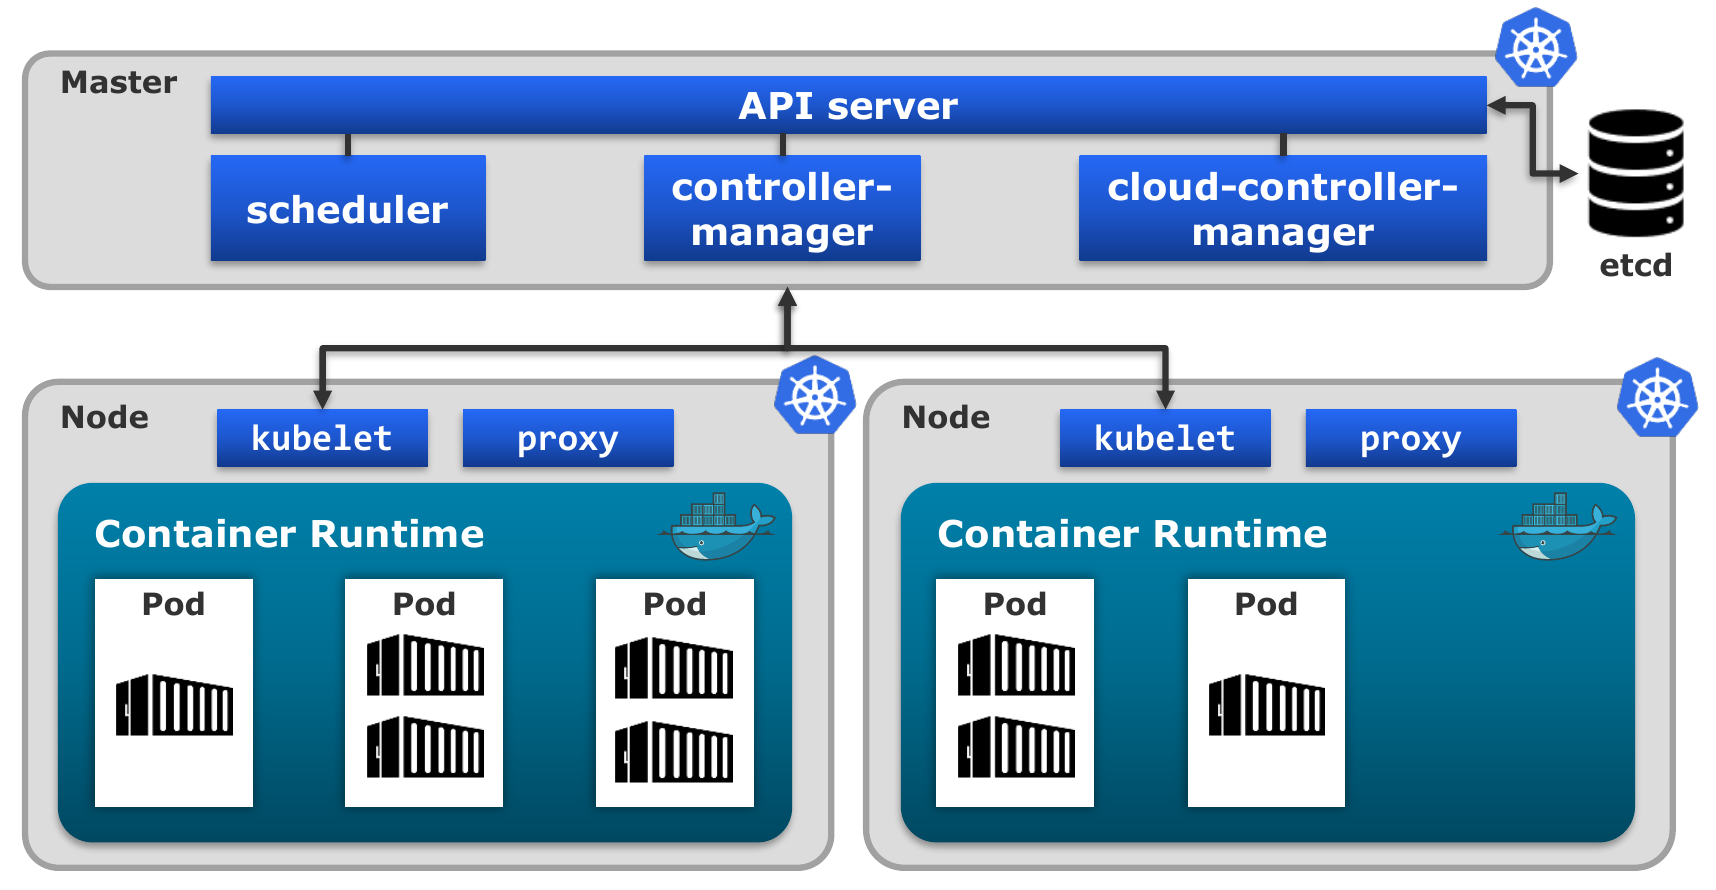
\includegraphics[width=\linewidth]{k8s-architecture}
    \caption{\Gls{kubernetes} architecture}
    \label{fig:kubernetes-architecture}
  \end{figure}

  The \gls{kubernetes} master components provide the cluster's control plane.
  They typically run only on one node, which does not run application pods.
  However, the components can be executed on any node in the cluster.
  The master components include
  (i) the \texttt{kube-apiserver} that exposes the control options to the user and other software,
  (ii) an \texttt{etcd}~\cite{etcd} instance as store for all cluster data,
  (iii) the \texttt{kube-scheduler}, which schedules newly created pods to the nodes in the cluster,
  (iv) the \texttt{kube-controller-manager}, which runs node and pod controllers, and
  (v) the \texttt{cloud-controller-manager} to interact with the underlying cloud providers~\cite{kubernetes}.

  % https://kubernetes.io/docs/concepts/overview/working-with-objects/kubernetes-objects/
  For the declarative configuration and management of the application, \gls{kubernetes} employs the \gls{kubernetes} object model.
  All entities of the \gls{kubernetes} runtime are represented as description objects.
  The entirety of those objects represents the cluster state.
  Each object consists of three parts:
  (i) the object's metadata, such as name, version or labels,
  (ii) the object \texttt{spec}, which describes the desired state for the object and is provided by the user, and
  (iii) the object \texttt{status}, which describes the actual state of the object.
  Users of \gls{kubernetes} therefore only provide the object's metadata and \texttt{spec} to declare the desired deployment of their containerized applications on nodes and policies around how the application should behave.
  \Gls{kubernetes} will constantly update the \texttt{state} of the objects according to the observed cluster state and take corrective actions in the cluster to ensure that the cluster state matches the desired one declared in the objects' \texttt{spec}~\cite{kubernetes}.

  % https://kubernetes.io/docs/concepts/overview/working-with-objects/labels/https://kubernetes.io/docs/concepts/overview/working-with-objects/labels/
  % should I describe labels as well?
